
\def\theThemeTitle{Sottomarino telecomandato da remoto (ROV)}

\def\theThemeDescription{%
Un sottomarino telecomandato da remoto (ROV) è soggetto alla spinta di galleggiamento, alla spinta longitudinale dei motori di poppa e a quella dei motori di prua. La navigazione del veicolo richiede di stabilizzare la posizione della prua del veicolo attraverso la misura della stessa.
}

\def\thePicture
{
\begin{center}
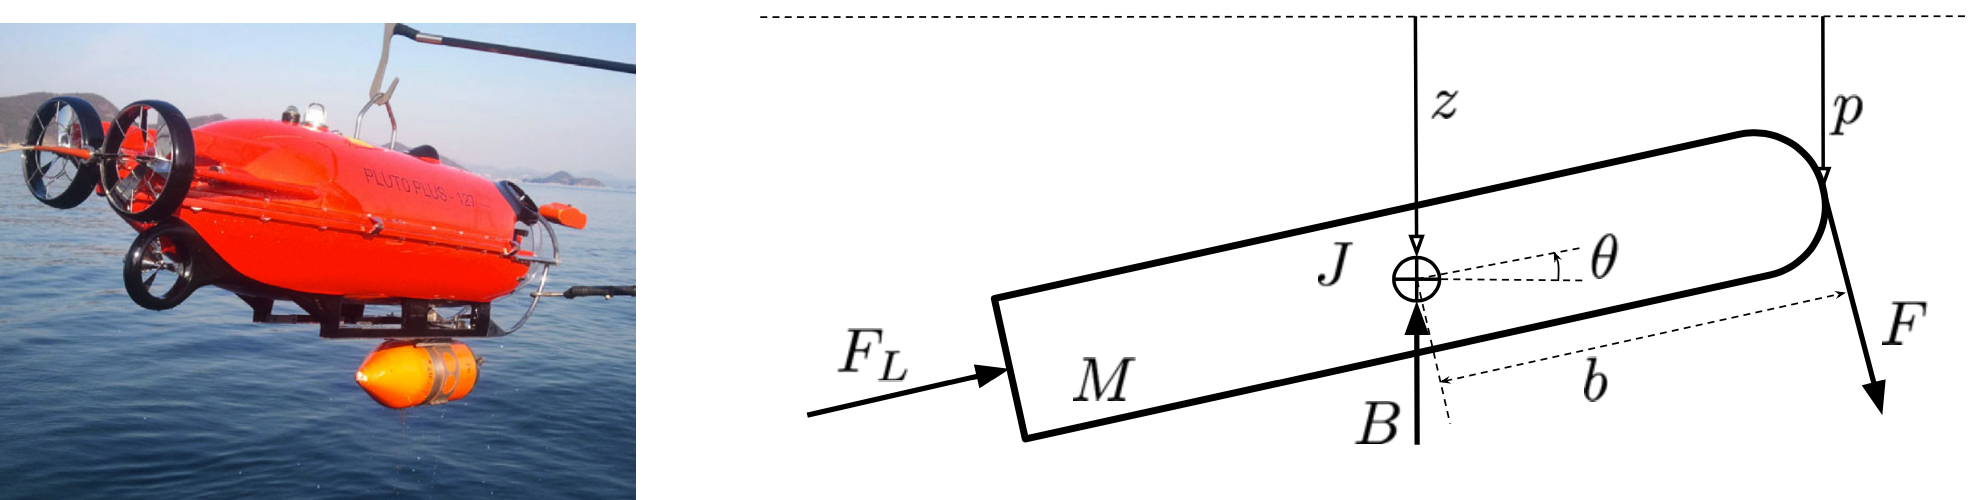
\includegraphics[width=0.6\textwidth]{img/rov.png}
\end{center}
}

\def\theModel
{
\begin{equation}
\label{eq:model}
\begin{array}{rcl}
M \, \ddot z & = & F \, \cos\vartheta - k_z \, \dot z \cos\vartheta - F_L \sin\vartheta - B \, , \\
%
J \, \ddot\vartheta & = & -k_r \dot\vartheta - k_\vartheta \sin\vartheta - F \, b \, , \\
%
y & = & z - b \sin\vartheta \, .
\end{array}
\end{equation}
}

\def\theVariables
{
\begin{center}
Tabella~$1$ - Variabili e altre funzioni\\[5pt]
%
\begin{tabular}{ |p{1.2cm}||p{5.5cm}| }
\hline
Variab. & Descrizione\\
\hline\hline
$z$ & profondità del centro di massa dal pelo d'acqua [m]\\
$\vartheta$ & angolo di beccheggio [rad]\\
$F$ & (ingresso) propulsione dei motori di prua [N]\\
\hline
\end{tabular}
\end{center}
\vfill 
}

\def\theParameters
{
\begin{center}
Tabella~$2$ - Parametri\\[5pt]
%
\begin{tabular}{|p{1.1cm}||p{5cm}|p{1.5cm}|}
\hline
Param. & Descrizione & Valore\\
\hline \hline
$M$ & massa della sottomarino [kg] & $580$\\
$J$ & inerzia laterale del sottomarino [Nms$^2$] & $560$\\
$B$ & spinta di galleggiamento [N] & $20$\\
$F_L$ & spinta di propulsione longitudinale [N] & - \\
$b$ & distanza centro di massa -- prua [m] & 1.2\\
$k_z$, $k_r$ & coefficienti degli attriti viscosi [Ns/m], [Nms] & $133$ e $168$ \\
$k_\vartheta$ & constante di leva [Nm] & 143 \\
\hline
\end{tabular}
\end{center}
}

\def\theRequirements
{
\begin{center}
Tabella~$3$ - Condizioni di equilibrio e Requisiti\\[5pt]
\begin{tabular}{ |p{2.7cm}||p{11cm}| } 
\hline
Equilibrio (H1) & Angolo di beccheggio $\bar\vartheta = \pi/6$~[rad] e spinta di galleggiamento $B = \bar B$; $\bar z$, $\bar F$ e $\bar F_L$ da determinare.\\
\hline\hline
Requisito (R1) & Inseguimento perfetto di riferimenti costanti per la variazione dell'uscita, con un tempo di risposta non superiore a $45$~s ed eventuali oscillazioni entro il $5\%$ dal valore di regime.\\
\hline
%Requisito (R2) & I disturbi sinusoidali in alta frequenza ($d(t) = A_\omega \sin(\omega t)$, con $|A_\omega| <0.5$ e $\omega > 50$ rad/s) devono essere attenuati di $40$~db.\\
%\hline
\end{tabular}
\end{center}
}

\def\afTheoryQuestion{{\em Domanda da definire}}
